\documentclass[12pt, a4paper]{article}
\usepackage{verbatim} 
\usepackage{subfig}
\usepackage{wrapfig}
\usepackage{listings}
\usepackage{array}
\usepackage[utf8]{inputenc}
\usepackage{todonotes}
\usepackage{newtxtext}
\usepackage{blindtext}
\usepackage{enumitem}
\usepackage{graphicx}
\usepackage{pdflscape} % For landscape pages
\usepackage{float}     % For ordering images and text accordingly
\usepackage[colorlinks = true, urlcolor  = blue]{hyperref}
\graphicspath{ {./images/} }
\usepackage{biblatex}
\addbibresource{Bibliography.bib}

\usepackage{hyperref}
\hypersetup{
    colorlinks=false, % Set to false if you don't want colored links
    linkcolor=blue,   % Color of links to internal documents
    filecolor=magenta, % Color of file links
    urlcolor=cyan     % Color of external links
}

\setlist[itemize]{itemsep=2pt, parsep=0pt}
\setlength{\arrayrulewidth}{0.3mm}
\setlength{\tabcolsep}{10pt}
\renewcommand{\arraystretch}{1.5}

%\setcounter{secnumdepth}{2}

\begin{document}
\begin{titlepage}
        \vspace*{-7em}
        \hbox{\hspace{14em}
\includegraphics[width=0.80\textwidth, ]{ITU_logo_UK.jpg}}
        \vspace*{4em}
    \begin{center}
        \centering 
        \vspace*{0.5cm}
        \LARGE
        \textbf{DevOps, Software Evolution and Software Maintenance: Exam Project}

        \vspace{1.5cm}
        
        \large
        \begin{center}
        \begin{tabular}{ |c|c| } 
        \hline
        \multicolumn{2}{|c|}{Group C}\\
        [0.5em]
        \hline
        Mathias Gleitze Hoffmann & mglh@itu.dk \\ 
        Martin Lupa Groppelli & mlup@itu.dk \\ 
        Anne Sofie Rasmussen & soad@itu.dk \\ 
        Cecilia Maria Fröhlich & cefr@itu.dk \\ 
        Tomas Federico Maseda & tofm@itu.dk \\ 
        Eleonora Borovic & eleb@itu.dk \\ 
        \hline
        \end{tabular}
        \end{center}
         
        \vspace{1cm}
        \normalsize

We have received the source code for a miniature version of X (formerly known as Twitter) in Python, for us to rewrite using another programming language. From there we have been asked to containerize our application, create a database, set up infrastructure using code, add a CI/CD chain, add logging and monitoring, and add container orchestration to enable our application to run in a distributed manner.

        \vfill

        
        KSDSESM1KU\\
        Spring, 2024
             
    \end{center}
\end{titlepage}

\pagenumbering{roman}
\setcounter{secnumdepth}{2}
\setcounter{tocdepth}{2}
\tableofcontents
\newpage
\pagenumbering{arabic}

\section{Systems}
\subsection{Design and architecture} \label{Design of the CSharp-MiniTwit application}
% We have decided to convert the given source code into an application called 'Csharp-Minitwit' written in C\#. We have chosen C\# for its well documented ecosystem and robustness, due to it being statically and strongly typed, and we have chosen to build our app using the NET 8.0 runtime, as it is the latest long-term supported release (end of support Nov. 2026)\cite{netcoresupport}.

% The application itself requires a database for storing users, messages, followers and metadata. For this we have chosen to connect to a PostgreSQL using Entity Framework Core (an ORM), making subsequent database alterations and migrations easy. In Figure \ref{fig:architecture} we have shown the architecture of the system. 

We have developed 'Csharp-Minitwit' using C\# and the .NET 8.0 runtime, chosen for its strong, statically typed ecosystem and long-term support.\cite{netcoresupport} The application uses the ASP.NET Core framework\cite{aspnetcoreintro2023}, with razor pages for rendering HTML pages, and we are following a Model-View-Controller (MVC) pattern and dependency injection, for easier maintainability and testability. We use PostgreSQL with Entity Framework Core for database management (an ORM), making subsequent database alterations and migrations easy. Below we will show the design and architecture of our system through the module viewpoints presented by Christensen et al.\cite{viewpoint} 

\subsubsection{Module Viewpoint}
In 'Csharp-Minitwit', the main modules include controllers, Models, Views, Services and Repositories. In Figure X, the dependencies between the modules can be seen. If we look into xxxx, it is apparent that the controller is heavily dependent on other modules, as illustrated in figure xx. 

\todo{Package diagram}

\subsubsection{Component \& Connector Viewpoint }
We will cover the Component \& Connector viewpoint under point 1.3. Elaborating on the interaction of subsystems.  

\subsubsection{Allocation Viewpoint}
% The purpose of the allocation viewpoint is to show how software elements are mapped to platform elements. 
%Figure \ref{fig:architecture} shows a full view of our deployment.
Figure \ref{fig:architecture} shows the infrastructure in our system.
It can be seen, how he application is hosted on DigitalOcean. We have a Docker Swarm Cluster to orchestrate containers and use Terraform for automating provisioning and configuration of the infrastructure.

\todo{elaborate on the elements. Refer directly to the figure}

\begin{figure}[H]
    \centering
    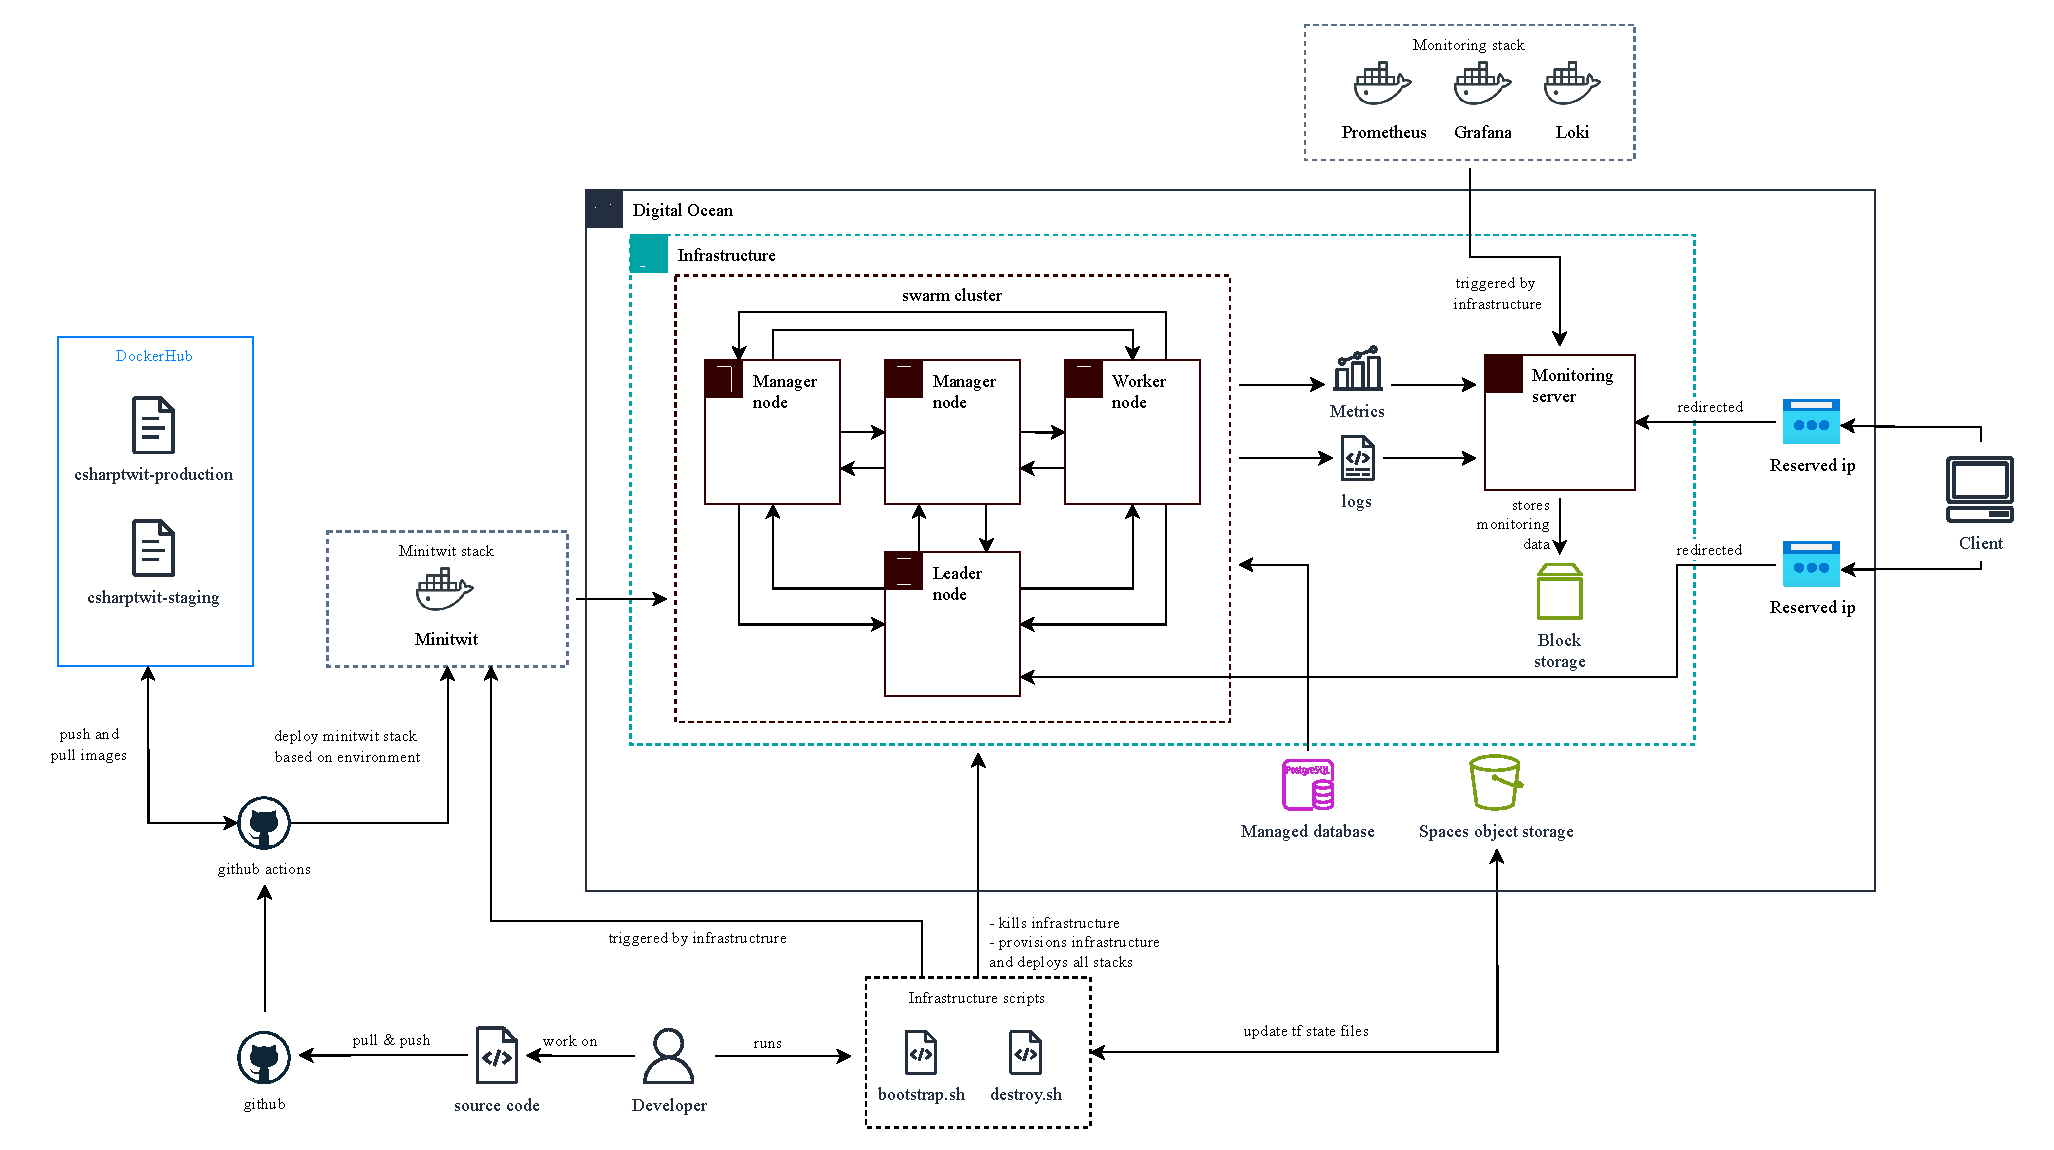
\includegraphics[width=1.0\textwidth]{figures/devops-architecture-architecture_v2.pdf}
    \caption{System Architecture Diagram, see large scale in Appendix \ref{apendix:systems-architecture}}
    \label{fig:architecture}
\end{figure}

\subsection{Dependencies and technologies}
\subsubsection{Application Dependencies}
% probably this info can be presented in tables with three columns (dev, staging, prod) and "X" pointing to the environment in which each is used.
Dependencies are handled using dotnet's package manager, NuGet:
\begin{itemize}
    \item Npgsql.EntityFrameworkCore.PostgreSQL 
    \item OpenTelemetry.Exporter.Prometheus.AspNetCore (exports telemetry data to Prometheus)
    \item OpenTelemetry.Extensions.Hosting
    \item Microsoft.EntityFrameworkCore (ORM)
    \item Serilog (structured logging library)
    \item Swashbuckle.AspNetCore (auto-generated Swagger documentation)
\end{itemize}

\subsubsection{Technologies used}
A quick overview of the technologies used:
\begin{itemize}
    \item \textbf{GitHub}: Code repository, versioning and project management.
    \item \textbf{SonarCloud}: ensuring quality in the code.
    \item \textbf{CodeClimate}: Quality analysis.
    \item \textbf{dotnet format}: Automatic formatting.
    \item \textbf{HadoLint}: Linting Docker file.
    \item \textbf{Digital Ocean}: hosting of virtual servers, databases and volumes.
    \item \textbf{Terraform}: provisioning and management of infrastructure on Digital Ocean.
    \item \textbf{Docker}: containerization of the application for deployment.
    \item \textbf{Prometheus}: monitoring system and time series database that collects metrics.
    \item \textbf{Loki}: log aggregation system integrated with Grafana for viewing logs.
    \item \textbf{Grafana}: visualization of metrics and logs.
\end{itemize} 
\subsubsection{Versioning and CI/CD}
% The application is versioned, tested, quality assured and deployed using
% GitHub. Our group has been following the Gitflow workflow to avoid merge conflicts, and ensure tractability. Gitflow also allows us to have a 'develop' and a 'main' branch, enabling us to easily set up a staging server, for integration testing.

% Our GitHub repository is also used for project management, creating issues and documentation. Deploying our application to our servers is done using GitHub actions, creating Docker images and pushing them to the relevant environment. GitHub actions also runs unit tests, formats our source code using 'dotnet format' and analyzes it using SonarCloud and CodeClimate.\\\\
% GitLab would have been a good alternative, however the whole group already have GitHub accounts and use it for personal projects — GitLab supports all the same features but is known for having a stronger focus on DevOps and CI/CD\cite{gitlabvsgithub}. GitLab allows for free self-hosting. 

Our CI/CD pipeline uses GitHub for versioning, issue tracking, and project management. GitHub Actions automate deployments, run unit tests, format code with 'dotnet format', and analyze it with SonarCloud and CodeClimate. We use Gitflow workflow for branch management, supporting staging and production environments.

\subsubsection{Cloud provider}
% We have chosen DigitalOcean as our cloud provider, running our application on provisioned virtual machines that we manage our selves. DigitalOcean has been chosen for the sole reason that they offered \$200 in credits for students — enough for the entire project.\newline 
% Since we are not using managed application services, pretty much any cloud provider would suit our needs. Had we gone with managed services, Azure would have been a good alternative due to its integrations for ASP.Net.

DigitalOcean hosts our virtual machines, chosen for its \$200 credits for students. Any cloud provider could suffice as we manage our VMs independently.

\subsubsection{Provisioning}
% For provisioning we use Terraform, which has been chosen specifically for it being declarative. The Terraform scripts are run using the 'bootstrap.sh' script, which takes a single parameter; 'production' or 'staging'. This in turn provisions our entire system (except the database) and pushes the corresponding docker image to the Docker Swarm.

Terraform, chosen for its declarative nature, provisions our infrastructure. The 'bootstrap.sh' script, which takes a single parameter; 'production' or 'staging'. This in turn provisions our entire system (except the database) and pushes the corresponding docker image to the Docker Swarm.

\subsubsection{Database}
As mentioned, the application uses a PostgreSQL database. We have opted to go with a managed database, for simplicity and to delegate reliability issues to DigitalOcean. A single vertically scaled database will be able to handle many concurrent users. If we needed to scale up substantiably, we would likely have to switch to a specialized distributed database system like Kafka, which the real X uses\cite{kafka}.

% We use a managed PostgreSQL database for simplicity and reliability. For scaling, we would consider a distributed database system like Kafka.

% \subsubsection{Monitoring and logging}
% We use Prometheus in a pull-based configuration for business monitoring. This was implemented as part of the exercises and has been kept for that reason. We also use DigitalOcean's website for infrastructure monitoring, displaying CPU, memory and disk usage. We have no alarms / emails set up.\\\\
% For logging we use Loki, which is inspired by Prometheus and chosen for that same reason\cite{Loki}.\\\\
% Grafana is used to display Prometheus data as a dashboard, and to query the logs from Loki.

% We use Prometheus for monitoring, DigitalOcean for infrastructure monitoring, it was introduced in exercises, and has been kept since. We have Loki for log aggregation, and Grafana for data visualization. Loki is inspired by Prometheus and chosen for that same reason\cite{Loki}.

\subsubsection{Containerization and container orchestration}
% The application is built as a Docker image through the CI/CD chain. From there it is deployed to an instance of Docker Swarm, using a compose file that connects our application with a Prometheus container. This setup has 2 replicas running on the swarm, more could be appliued, to scale the application if there is an increase in requests.\\
% The Grafana server is setup using standard Grafana, Prometheus and Loki images, composed together in a \texttt{docker-compose.yml}.\\\\
% The Docker Swarm is setup with 1 leader node, 2 manager nodes and 1 worker node. We only have a single worker node, as we have hit a max number of VMs, and we want to have both a staging and a production environment. To enable the leader node to crash and its role be taken by another node, it is required to have 2 manager nodes.\\\\

The application is containerized with Docker and deployed using Docker Swarm, set up with 1 leader node, 2 manager nodes, and 1 worker node. Grafana, Prometheus, and Loki are managed with a \texttt{docker-compose.yml} file.


\subsection{Interactions of subsystems}
Incoming requests to the application are handled by either the \texttt{APIController} or the \texttt{HomeController}. Both provide similar endpoint logic but are meant to be used by the simulator and regular users respectively. A request's path will match a specific endpoint, prompting the application to perform a corresponding database operation. For instance a POST request to \textit{/login} will invoke the \texttt{GetByUsername} method from the \texttt{userRepository} and request the user information through an SQL SELECT query. The ORM will map the results back to C\# objects, which the controller returns in the HTTP response to the user. 
Alng with this Prometheus and Grafana collect metrics to visualize. Data from logging is aggregated through Loki and Serilog. Below are two sequence diagrams showing how a user and the simulator interacts with our subsystems.\newline

In Figure \ref{fig:homecontroller} is a sequence diagram showing how a user successfully follow another user and gets a response from the system.\newline

\begin{figure}[H]
  \begin{center}
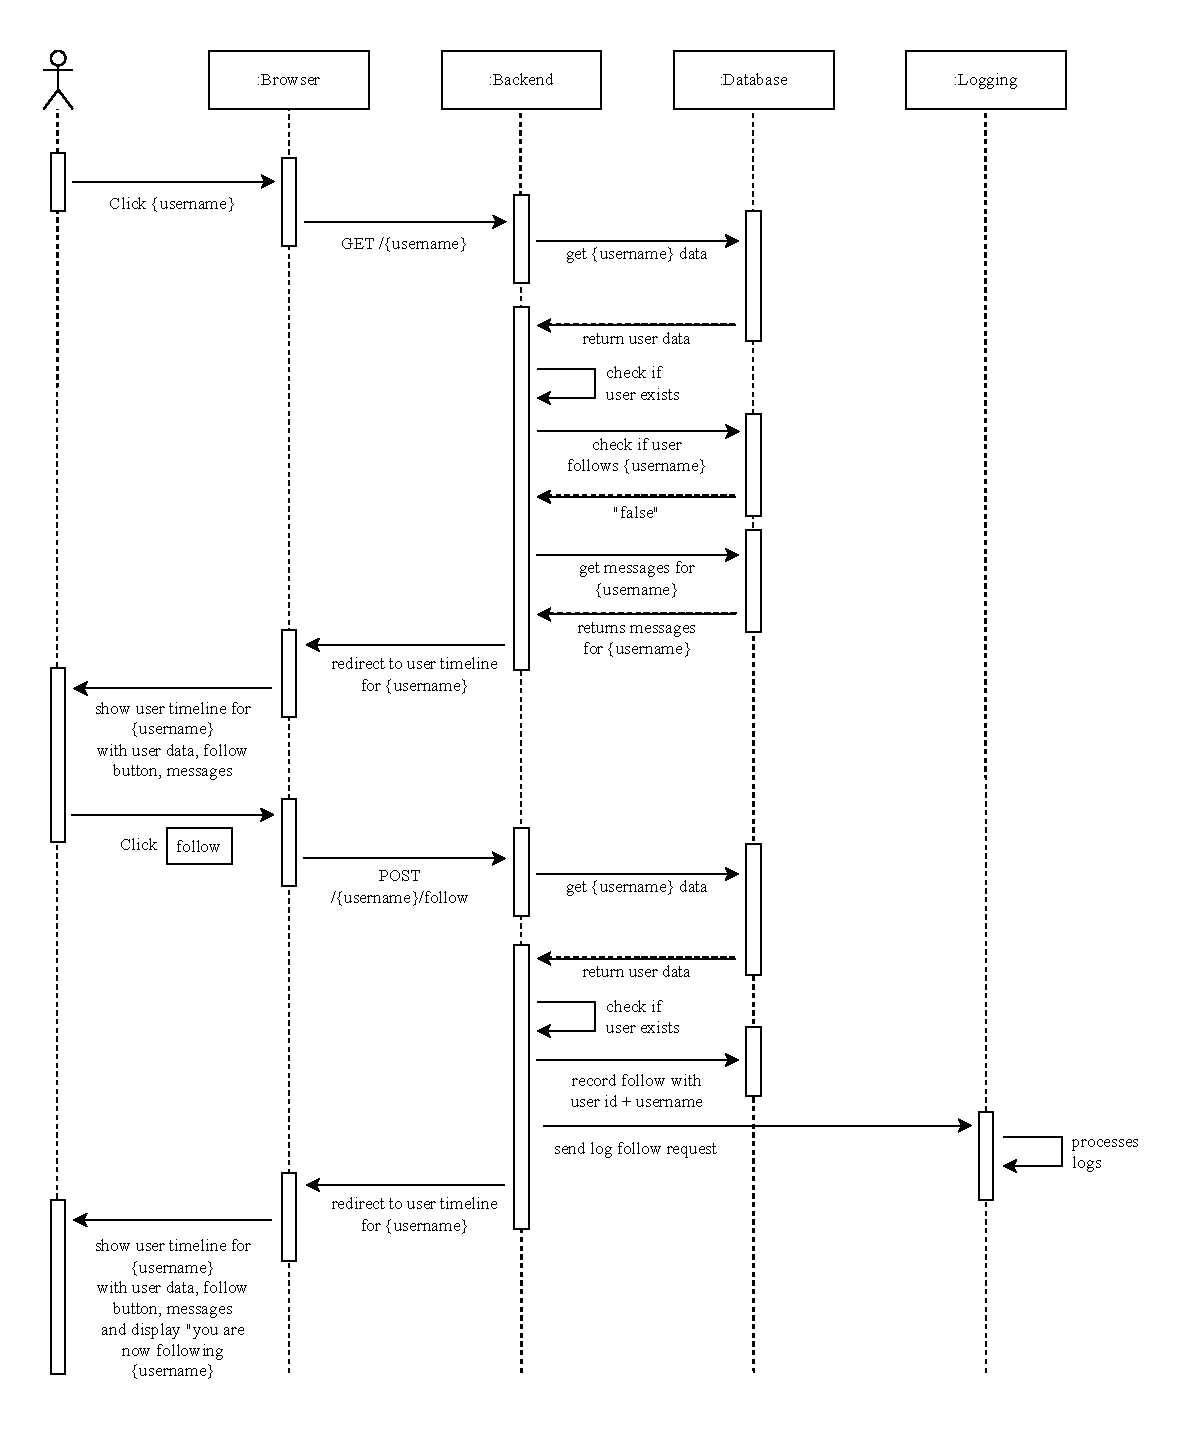
\includegraphics[width=\textwidth]{images/figures/Sequence-client.pdf}
    \caption{Sequence diagram of a successful follow scenario from user perspective.}
    \label{fig:homecontroller}
  \end{center}
\end{figure}

In Figure \ref{fig:apicontroller} is a sequence diagram illustrating how a request from the simulator is handled in the system.\newline

\begin{figure}[H]
  \begin{center}
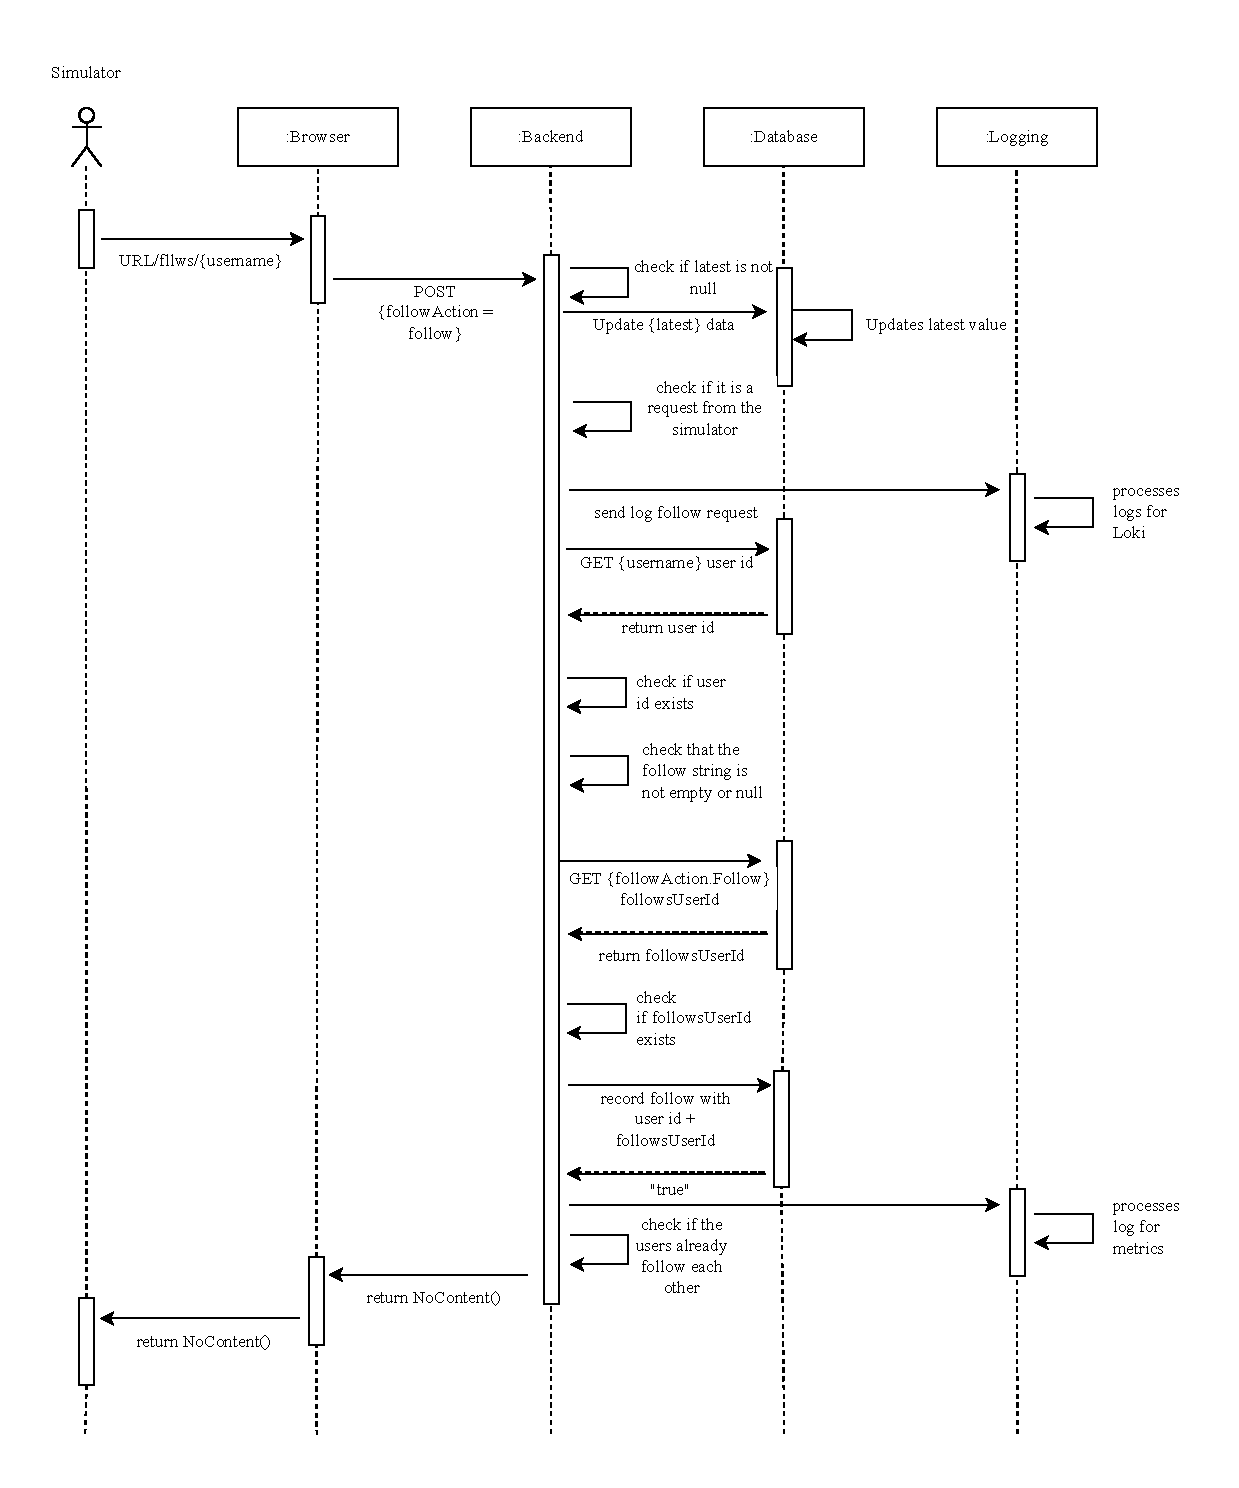
\includegraphics[width=\textwidth]{images/figures/Sequence-api.pdf}
    \caption{Sequence diagram of a successful follow scenario from the simulator over the API.}
    \label{fig:apicontroller}
  \end{center}
\end{figure}


\subsection{Current state of the systems}
The application is currently shutdown due to the limited amount of credits at DigitalOcean. 
Before this was done the application, had just been deployed with Terraform, implementing the functionality of the docker-swarm cluster. The application was fully functional on the last days of the simulator running, after this deployment.\newline

We have implemented different tools that can track the quality of our code including CodeClimate and SonarCloud.

\begin{figure}[H]
    \centering
    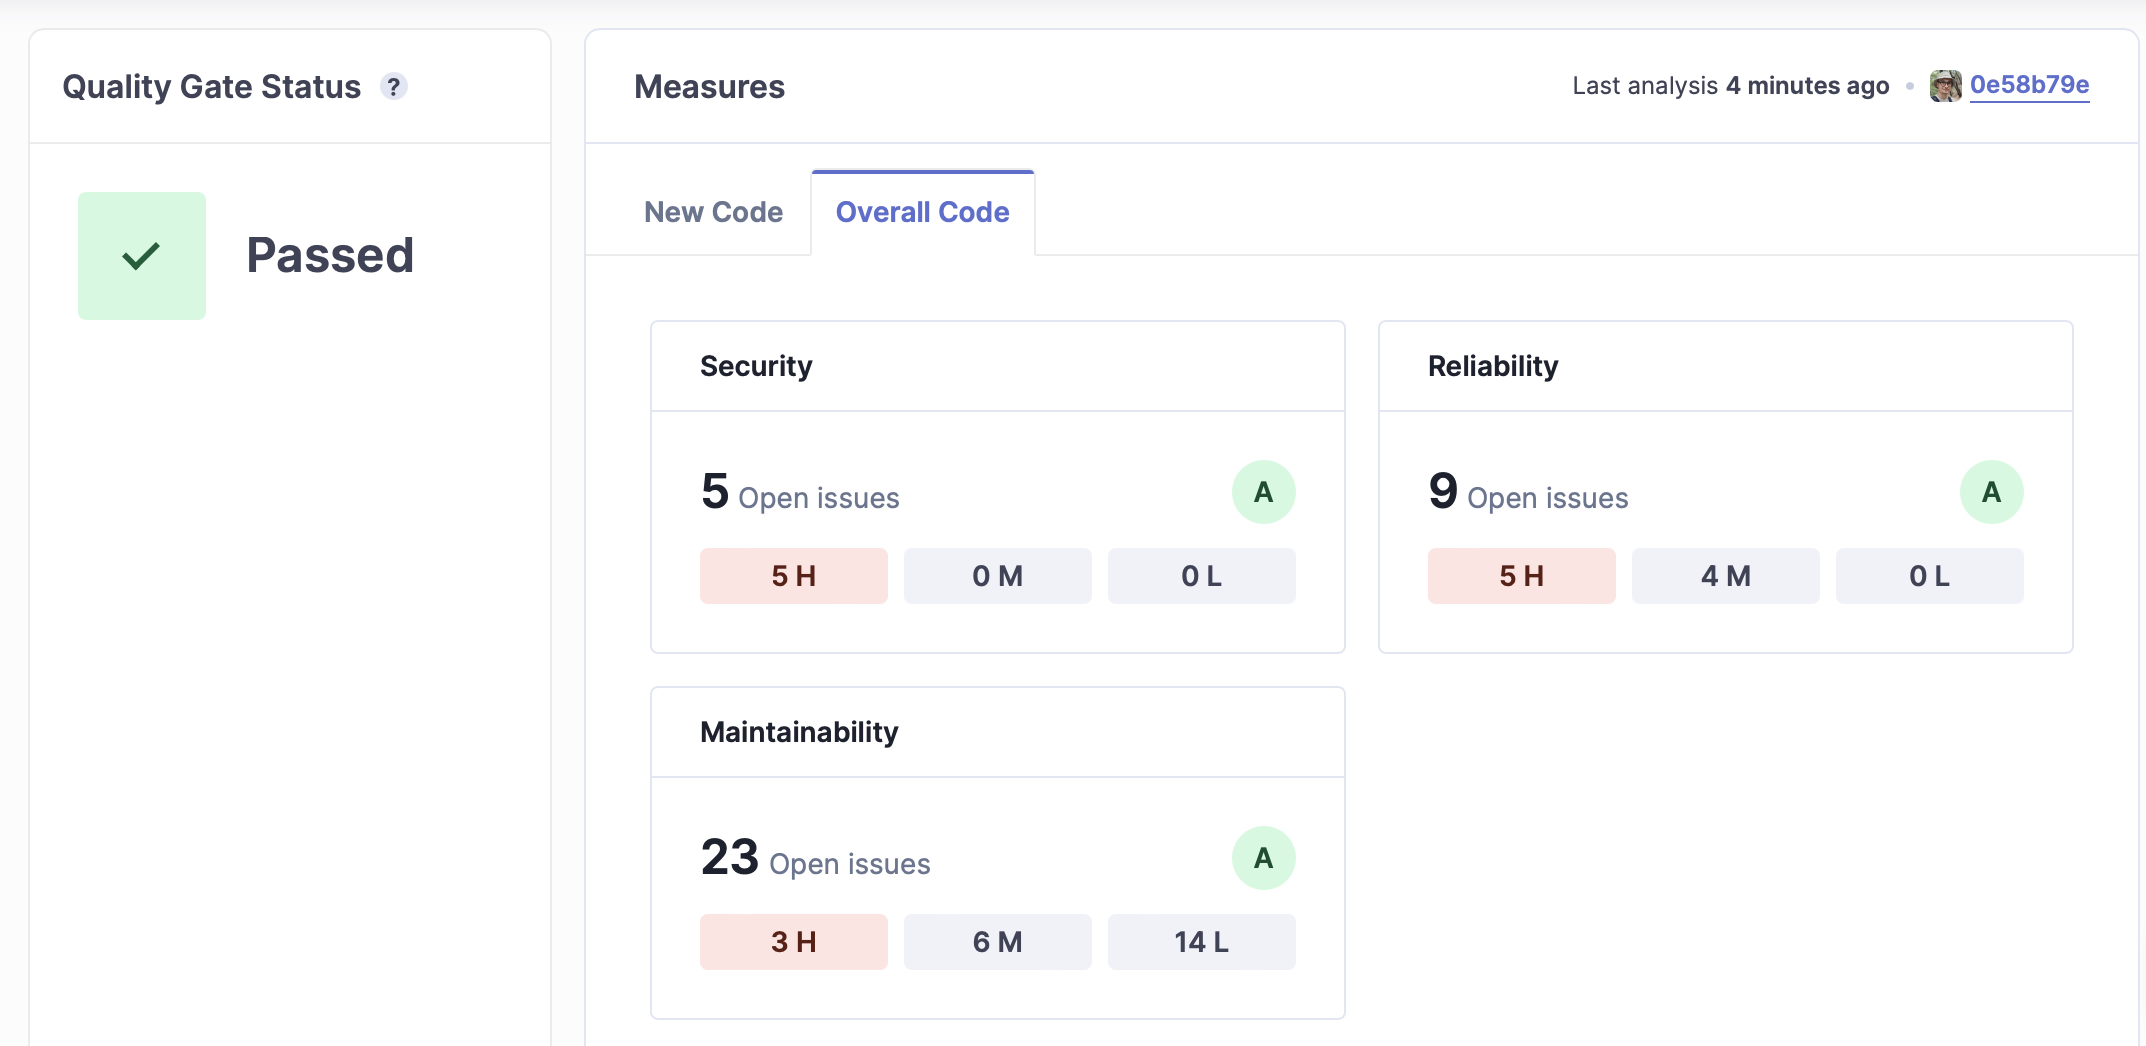
\includegraphics[width=\textwidth]{images/QualityGate.png}
    \caption{Screenshot of the latest SonarCloud Quality Gate}
    \label{img:qualitygate}
\end{figure}

\noindent Figure \ref{img:qualitygate} shows a screenshot of the latest quality gate state in SonarCloud. It displays, that there remains some open issues.  All of them have rating A, meaning that it has the lowest score when it comes to improving the software. \cite{codeclimate} When it comes to technical dept, we currently have 5\%, which improved after implementing the tools, as seen in Figure \ref{img:technical dept}. 

\begin{figure}[H]
    \centering
    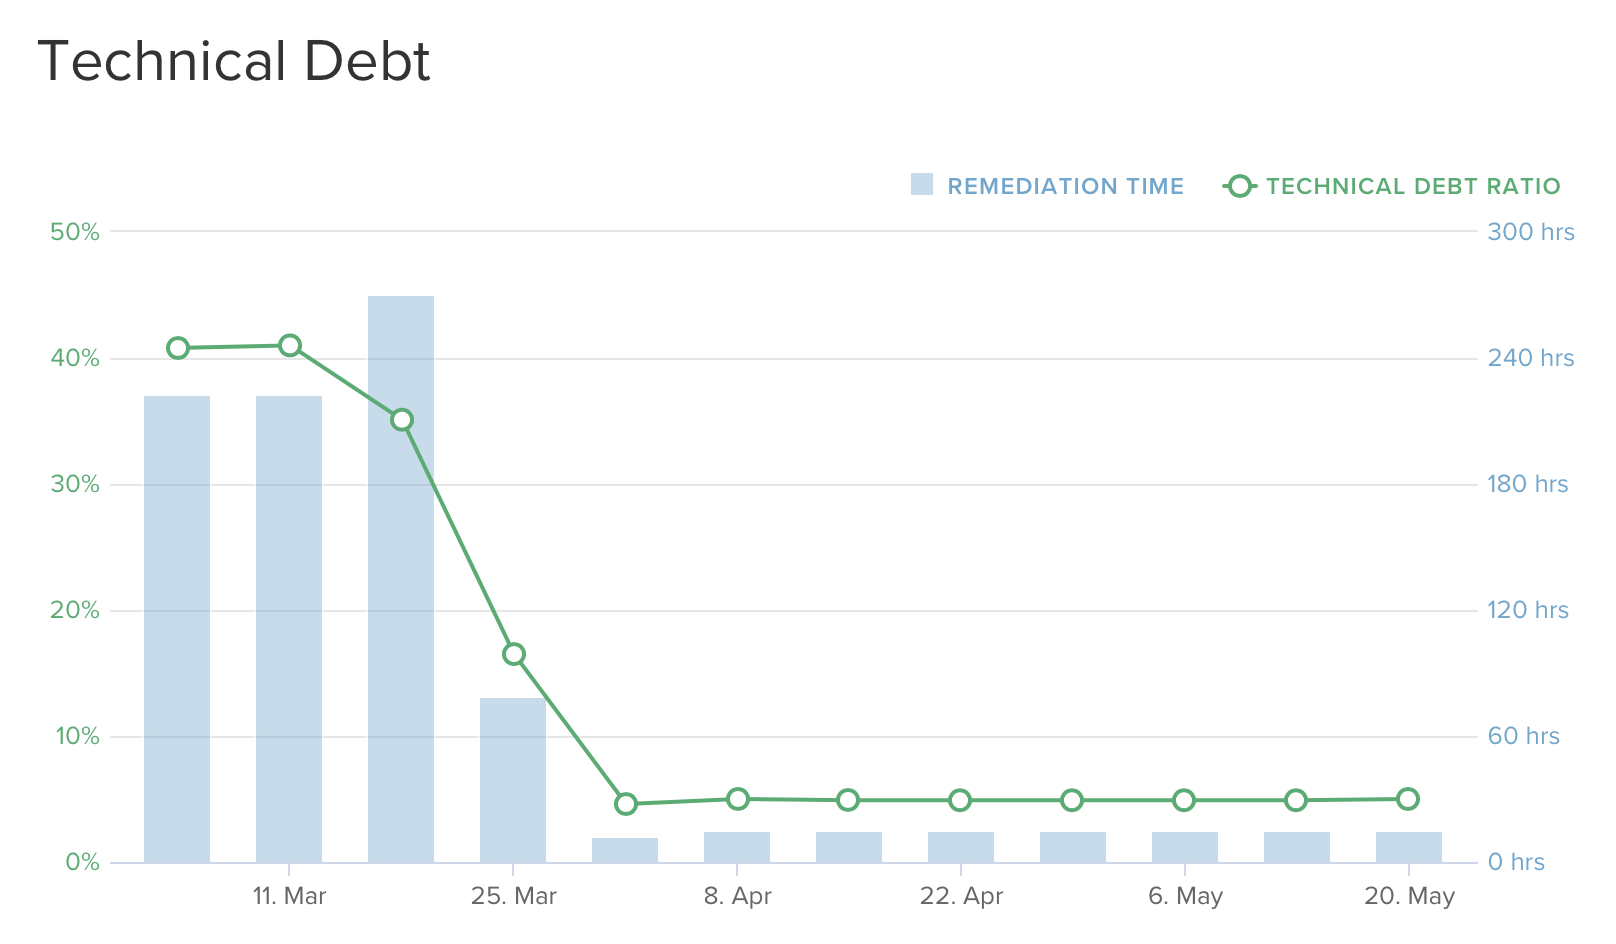
\includegraphics[width=\textwidth]{images/Technical Debt.png}
    \caption{Screenshot of the Technical Dept in our system, from CodeClimate}
    \label{img:technical dept}
\end{figure}



\newpage
\section{Processes}

% \subsubsection{Docker Swarm - Csharp-Minitwit application}
% When deploying a Docker Swarm cluster, a reserved IP is assigned to the manager node. Users will use this IP to send requests to the Csharp-Minitwit application. When receiving a request, the Docker Swarm cluster routes it through its routing mesh to one of the worker nodes running an instance of the Csharp-Minitwit application, which will process the request and serve a response.

\subsection{Tools and stages included in CI/CD pipelines}
\label{tools-and-stages-ci-cd}
% A complete description of stages and tools included in the CI/CD chains.
% That is, including deployment and release of your systems.
Our CI/CD pipelines are implemented using Github Actions. Our workflows are splitted in the following:

\subsubsection{quality.yml}
Triggered on pull request actions (opened, reopened, edited, synchronize, and ready for review). The main purpose is to run quality checks over the changes existing on the pull request branch. Figure \ref{fig:quality.yml} illustrates the stages of the quality workflow.

\begin{figure}[H]
    \centering
    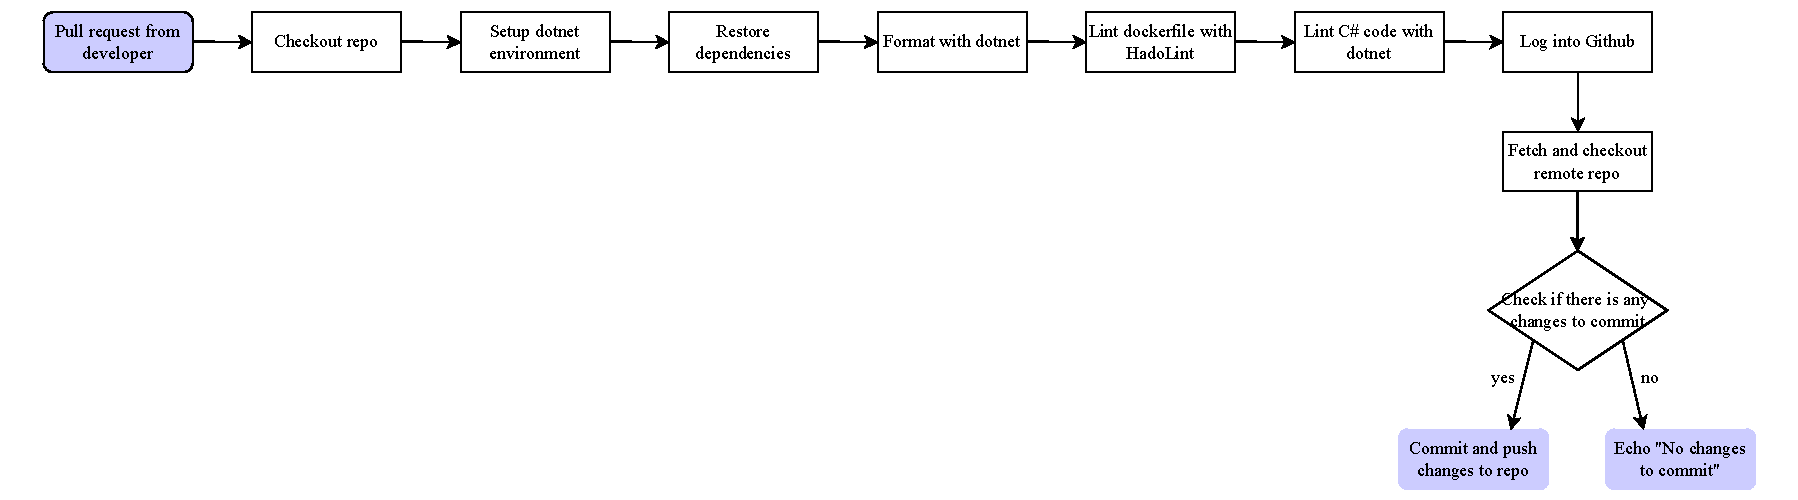
\includegraphics[width=\textwidth]{images/figures/Quality.pdf}
    \caption{Flowchart illustrating the stages of the quality workflow}
    \label{fig:quality.yml}
\end{figure}

\noindent  Tools used in quality.yml:

\begin{itemize}
    \item .NET SDK (for running dotnet commands)
    \item dotnet format (for automatic formatting)
    \item Hadolint (for Dockerfile linting)
    \item SonarQube (for code quality and security analysis)
\end{itemize}

\subsubsection{release.yml}
Triggered on pushes to \texttt{main} branch. It uses a base \texttt{release.config.js} file at the root of the repository and it is meant to automate the generation of releases and its changelogs through the use of conventional commit messages. Figure \ref{fig:release.yml} illustrates the stages of the release workflow.

\begin{figure}[H]
    \centering
    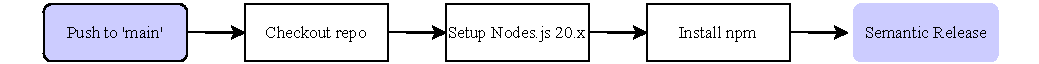
\includegraphics[width=\textwidth]{images/figures/Release.pdf}
    \caption{Flowchart illustrating the stages of the release workflow}
    \label{fig:release.yml}
\end{figure}

\noindent  Tools used in release.yml:
\begin{itemize}
    \item Node.js (for running npm and semantic-release)
    \item Semantic Release (for versioning and changelog management)
\end{itemize}

\subsubsection{deploy.yml}
Triggered on pushes to \texttt{develop} and \texttt{main}. It internally checks the targeted environment \texttt{(staging} or \texttt{prod)} retrieving the corresponding secrets,pushing the application image to Dockerhub and deploying to Digital Ocean. Figure \ref{fig:deploy.yml} illustrates the stages of the release workflow.

\todo{picture tomorrow}

\noindent  Tools used in deploy.yml:
\begin{itemize}
    \item Docker (login, build, push actions)
    \item SSH (for deploying to servers)
\end{itemize}

% \noindent When developers work on the source code, and merge the new features into the main branch, it triggers a deployment workflow that updates the application's Docker images on Dockerhub. A later step uploads the Terraform state files for infrastructure management, which pulls the updated images and initiates the infrastructure update process, deploying changes to Digital Ocean.

% \subsection{Organization of the repository}
% % Organization of your repositor(ies).
% % That is, either the structure of of mono-repository or organization of artifacts across repositories.
% % In essence, it has to be be clear what is stored where and why.
% The repository is organised in two main folders: csharp-minitwit and infrastructure. The first contains all application specific logic, while the second holds all infrastructure related configuration files.

% By organising the repository in this manner, there is a clear separation of concerns, making it easier to manage the project. Developers concerning with the development of the application do not need to understand the intricacies of the infrastructure and vice versa. 

% \subsubsection{csharp-minitwit}
% Main folders and files explained:
% \begin{itemize}
%     \item Controllers: APIController and HomeController handle all the logic for each endpoint.
%     \item Databases: contains the \texttt{schema.sql} and \texttt{minitwit.db} files used to initialise the database in the development environment.
%     \item Metrics: contain all metrics logic and configuration.
%     \item Middlewares: currently only a CatchAllMiddleware required to catch incoming requests and record metrics.
%     \item Models: these represent the way the data is shaped in the application. %I do not completely understand the division into api and DTOs. We should probably explain why.
%     \item Services: include the business logic and service layer components. ORM logic is reflected under Repositories.
%     \item Views: templates representing the user interface.
% \end{itemize}

% \subsubsection{infrastructure}
% Main folders and files explained:
% \begin{itemize}
%     \item archive
%     \item grafana
%     \item scripts
%     \item ssh\_key
%     \item stack
% \end{itemize}
    
    
% \subsection{Applied branching strategy}
% We have decided to use Gitflow branching model\cite{nvie2010git}. In this model the repository holds two main branches:
% \begin{itemize}
%     \item \texttt{main}: represents the main branch where the source code of HEAD is always production-ready.
%     \item \texttt{develop}: it serves as an integration branch where source code of HEAD always reflects a state with the latest delivered development changes for the next release.
% \end{itemize}
% Next to these main branches there are some other supporting branches, being \texttt{feature} the most widely used. feature branches are meant to be used to develop new features for future releases. They usually branch off and back to develop.

% \subsection{Applied development process and tools supporting it}
% % For example, how did you use issues, Kanban boards, etc. to organize open tasks
% To organise the development process and make work visible we decided to capitalise Github's built in Project tab, which provides an adaptable spreadsheet for tracking work, and which also integrates with Issues and Pull Requests. This tool provides a comprehensive visibility to the current state of each ticket and an easy-to-understand interface for developers and stakeholders.

% A new Issue is created to document a new requirement and is automatically shown in the Project board as a "Todo" item. When a team member is assigned to such issue, it is moved into the "In Progress" state. The development phase takes part, and when the issue is closed, it is automatically moved to the "Done" status in the board. Closing an issue as "not planned" takes the ticket to the "Aborted" status.

% \begin{figure}[H]
%     \centering
%     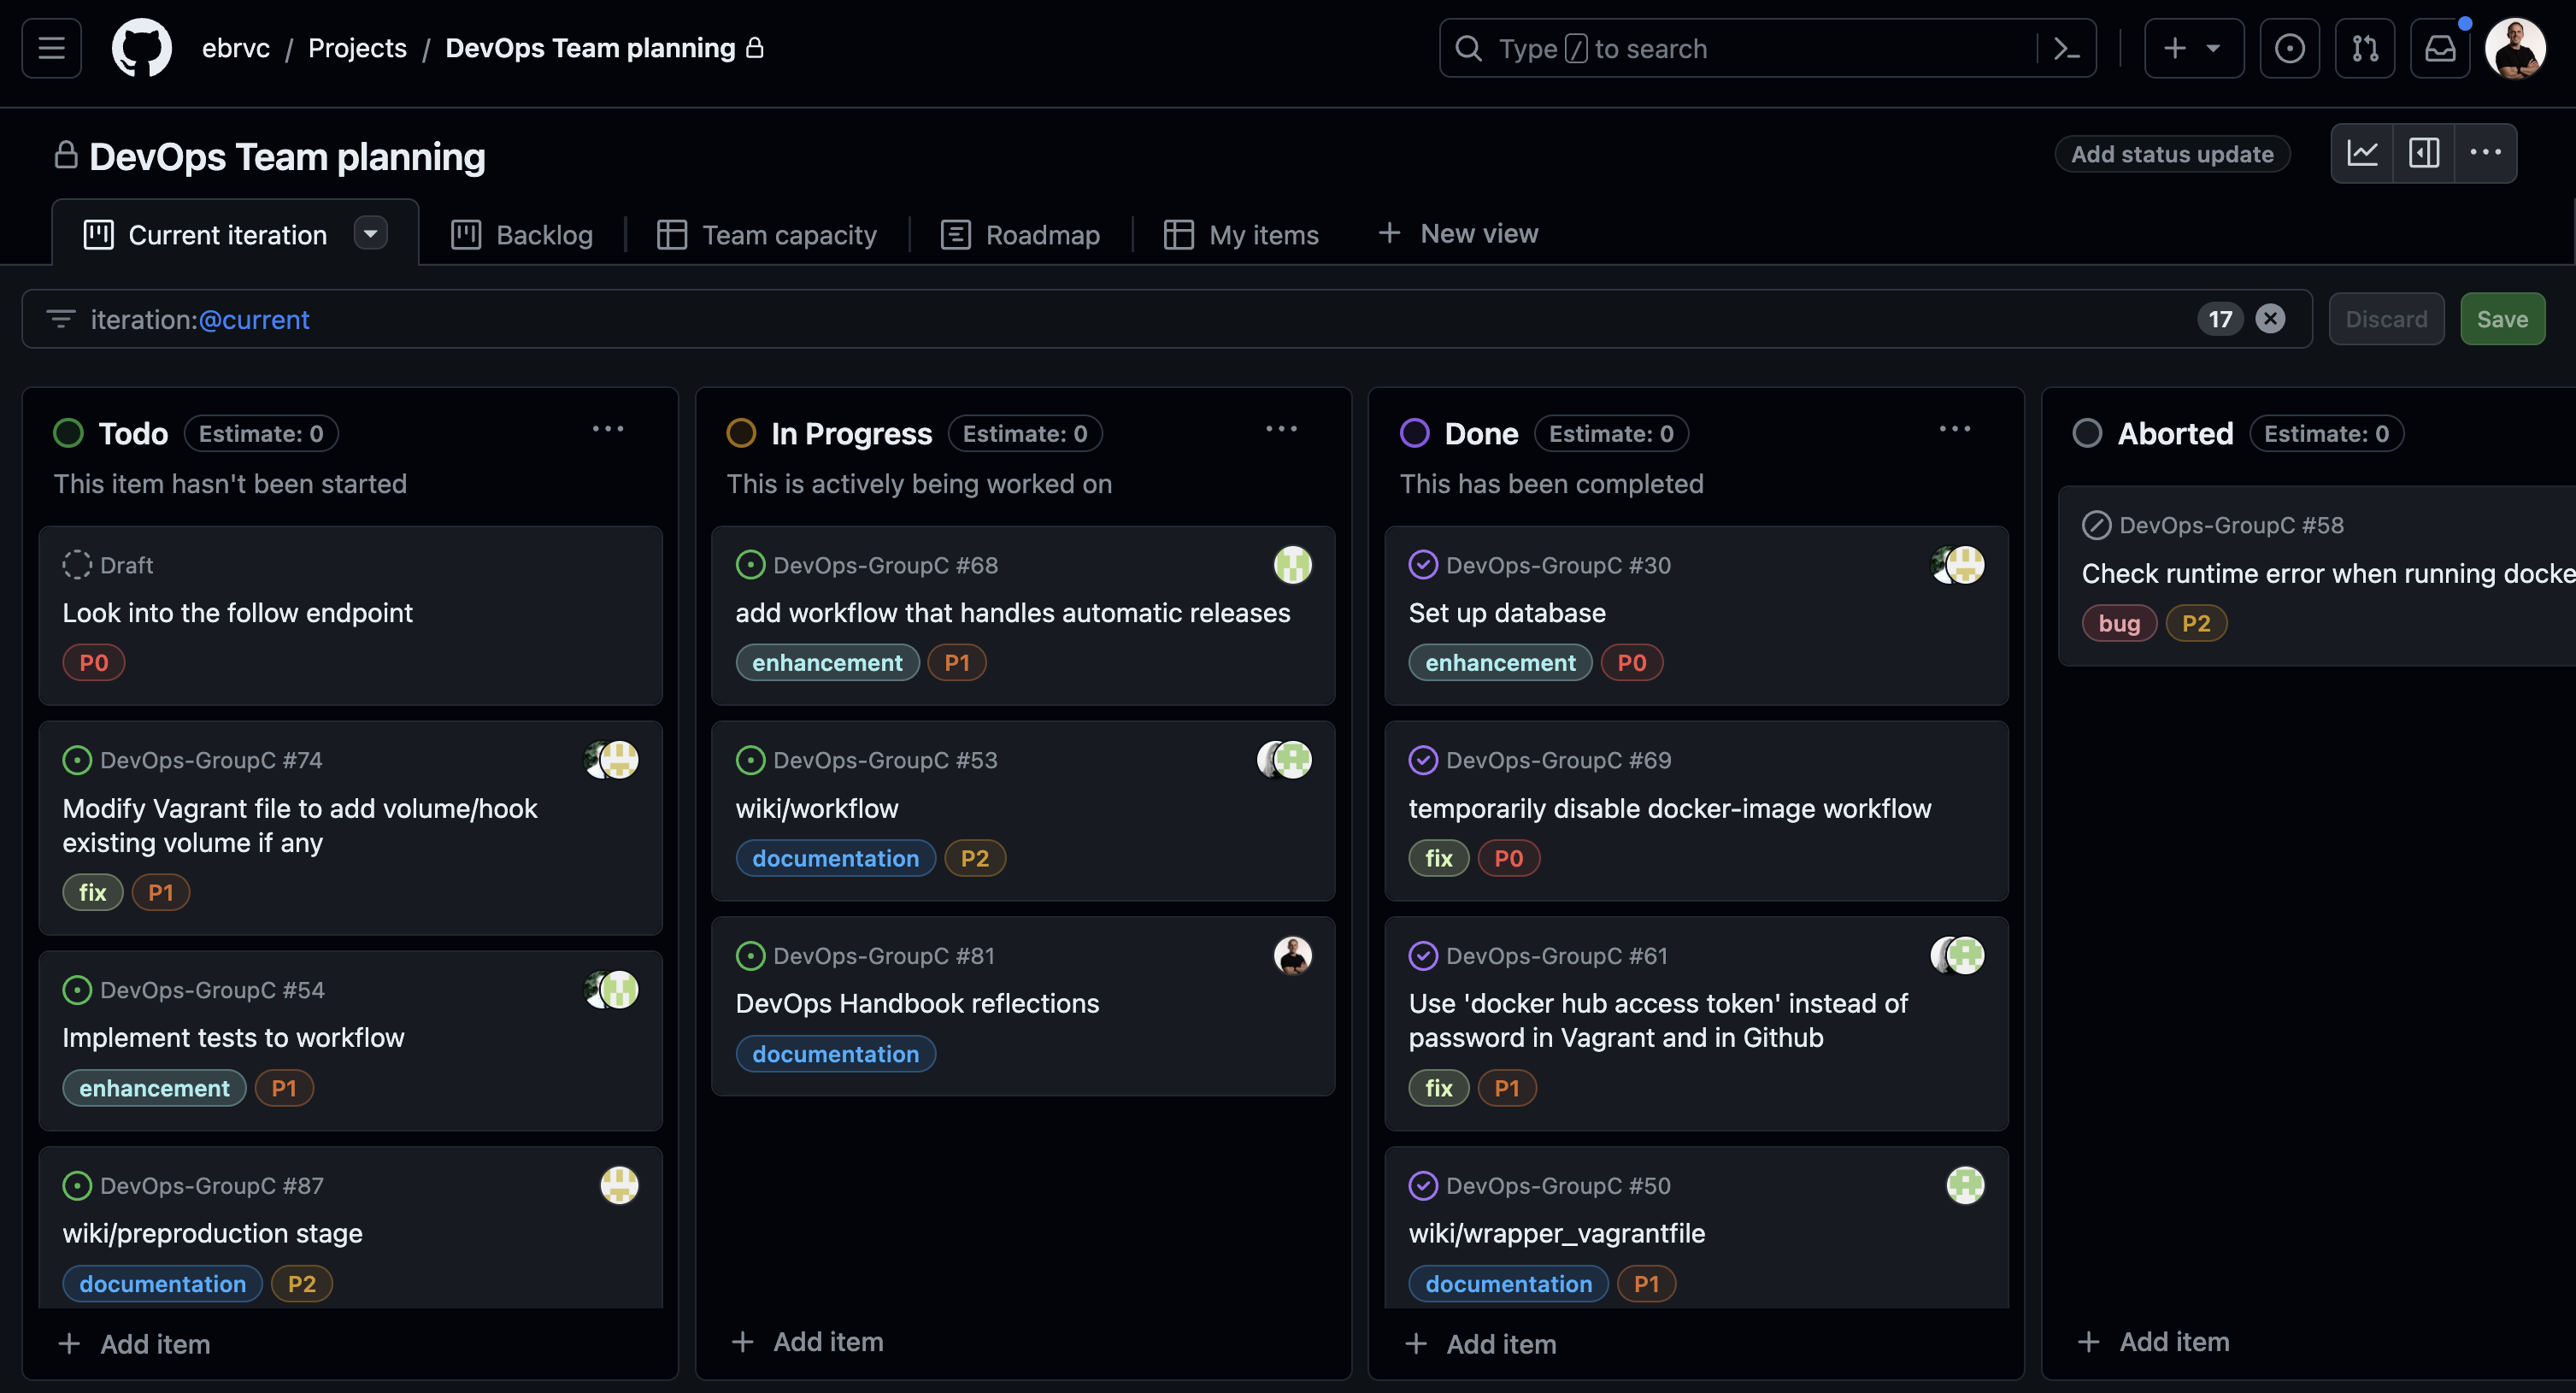
\includegraphics[width=\textwidth]{images/github-project-tracking.png}
%     \caption{Github's Project tracking tool}
%     \label{fig:github-project-feature}
% \end{figure}

\subsection{Monitoring}
% How do you monitor your systems and what precisely do you monitor?
Monitoring is conducted using a self-hosted instance of Grafana on a DigitalOcean Droplet. This instance receives metrics data from Prometheus servers attached to the application droplet. When the Csharp-Minitwit application processes a request that involves a metric method, the OpenTelemetry.Exporter.Prometheus.AspNetCore package collects and exposes these metrics on a \textit{/metrics} endpoint. A Prometheus server scrapes this endpoint at regular intervals. Prometheus is then used as a data source for Grafana, allowing us to visualize this information on a dashboard.\newline

Some of the data is also collected by querying the database on some specific indicators, such as:
\begin{itemize}
    \item Messages registered (application usage)
    \item Users registered (conversion)
    \item Follower registrations (users interaction level)
\end{itemize}

\subsubsection{Application monitoring}
The data is then used together with the build in packages to display, how the application is performing. We have chosen to monitor the following, as seen in Figure \ref{fig:grafana-dashboard}.
\begin{itemize}
    \item Rate of HTTP requests received per endpoint
    \item Total number of requests (last 24hs)
    \item Total count of errors per status code (last 24hs).
    \item Top 10 unhandled exception endpoints.
    \item Top 10 Requested endpoints (API).
\end{itemize}

\begin{figure}[H]
    \centering
    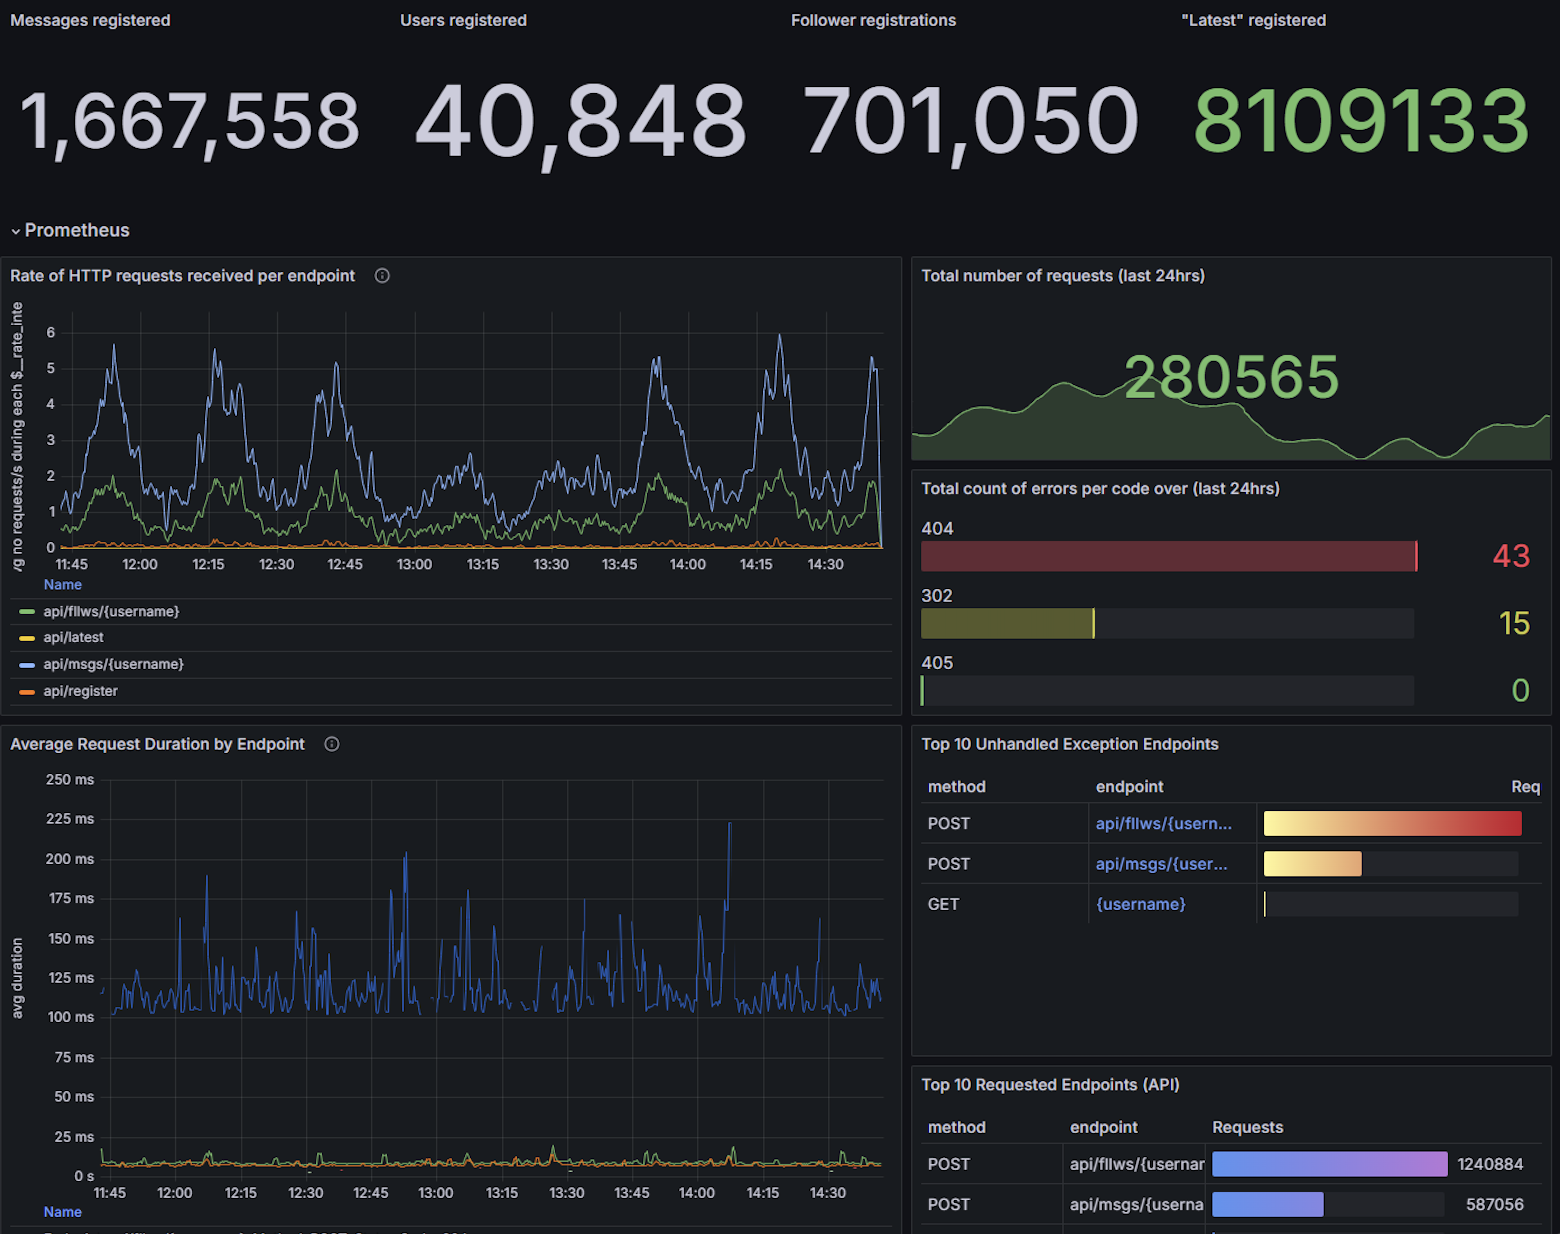
\includegraphics[height=0.9\textwidth]{images/Monitoring-latest.png}
    \caption{Snapshot of Grafana Monitoring Dashboard}
    \label{fig:grafana-dashboard}
\end{figure}

\subsubsection{Infrastructure monitoring}
Even though we haven't set this monitoring ourselves, Digital Ocean provides some out of the box monitoring for its droplets, such as CPU usage, memory usage, DISK I/O, Disk Usage, Bandwith, etc.

\subsection{Logging}
% What do you log in your systems and how do you aggregate logs?
Logging is configured through a log aggregation system called Loki, which acts as a Grafana datasource. These logs are pushed directly to Loki by using Serilog, a logging library for .NET applications. Serilog configures a C\# API that will receive the Csharp-Minitwit application logs and send them in a POST request to Loki's server. The structured representation of these Logs makes it easier to extract information from them at a later point. Loki can then be configured as a data source in Grafana to process and store these logs to be queried from a Dashboard.

We have chosen Loki due to its integration with Grafana and its simpler architecture, which requires less computational power and memory. This aligns perfectly with our Csharp-MiniTwit application. \newline

Below, we present the log events throughout our application:
\begin{itemize}
    \item Message posting
    \item User logging / Failure logging / Invalid username or password
    \item User logout
    \item User registering / Failure registering
    \item API requests that are not from the simulator
    \item API registering / Failure registering
    \item API message posting from users / Failure or incorrect usage of endpoint
    \item API retrieval of messages for a specific user / Failure in the retrieval
    \item API retrieval of followers for a specific user / Failure in the retrieval
    \item API follow/unfollow requests / Failure in the execution
    
\end{itemize}

\todo{Describe how we aggregate logs}



\subsection{Security assessment}

Having multiple assets, we have multiple threat sources.\newline 
We have the following assets:
\begin{itemize}
    \item Web application
    \item Database
    \item CI/CD
    \item Image repository
    \item Container orchestration
    \item Secrets
\end{itemize}

\subsubsection{Threat sources}

Web application: Runs on HTTP, making it vulnerable to data leaks and replay attacks. Possible XSS vulnerabilities due to HTML rendering.\\\\
Database: Usernames and emails are stored in clear-text; passwords are salted and hashed, to defend against rainbow-table attacks.
User IDs increment sequentially, which is not best practice.The same database credentials are used for both staging and production.\\\\
CI/CD: GitHub actions has access to all secrets.
We use the following NPM packages for release versioning:
\begin{itemize}
    \item "semantic-release-github-actions-tags": "\textasciicircum1.0.3"
    \item "semantic-release/git": "\textasciicircum8.0.0"
\end{itemize}

Images are publicly stored on DockerHub, with clear-text credentials on the staging server. The codebase is public on GitHub.\\\\
Other: Multiple open ports on servers, potentially including logging endpoints.

\subsubsection{Risk scenarios}

\begin{center}
\begin{tabular}{ |p{3.5cm}|c|c|c|p{2.5cm}| } 
 \hline
 Scenario & Probability & Impact & Risk & Strategy / Action\\ [0.5ex] 
 \hline
 An adversary listens to the non-encrypted data sent on our web application. This is possible because we use HTTP and not HTTPS
 & 5 & 5 & 25 & Get an SSL-certificate and redirect all traffic to HTTPS\\
\hline
 An adversary finds an open port on one of our nodes and gains access to our system & 3 & 5 & 15 & Run Nmap, close unused ports\\
 \hline 
 An adversary constructs a message that escapes HTML and runs code when rendered (XSS) & 3 & 5 & 15 & Sanitize user input\\
 \hline
  An adversary finds our Docker images online & 3 & 1 & 3 & Make image repository private\\ 
 \hline
 An adversary hijacks the cookie of a user & 1 & 2 & 2 & Unavoidable\\ 
 \hline
\end{tabular}
\end{center}


\noindent We have not had time to harden our system, due to our focus primarily being on making the infrastructure. 

\subsection{Scaling and upgrades}
Because we monitor our system we can see when there would be a need to scale our system up or down. Our strategy for scaling our system is to change the number of nodes in the terraform file minitwit\textunderscore swarm\textunderscore cluster.tf and run the bootstrap.sh script. Because the state of our system is kept in the Spaces Object Storage in DigitalOcean it would allow for a quick scaling of the number of nodes. 

Currently we do not have an automated process for upgrading the system, this would have to be done automatically. From our experience upgrading the initial python2 application to python3, we know that this is not necessarily easy process, where all dependencies has to be taken into account as well. 

% Applied strategy for scaling and upgrades

\subsection{AI-assistance}
AI tools have not been abandoned in our development process. The main AI consultancy has been with ChatGPT, which has primarily been used for debugging and providing advice on various issues. However, since our application is unique, the ChatGPT platform has limited resources specific to our application's actual processes. Instead, we found that the documentation for each dependency was more thorough and effective for problem-solving in our specific implementation.

\newpage

Having multiple assets, we have multiple threat sources.\newline 
We have the following assets:
\begin{itemize}
    \item Web application
    \item Database
    \item CI/CD
    \item Image repository
    \item Container orchestration
    \item Secrets
\end{itemize}

\subsubsection{Threat sources}

Web application: Runs on HTTP, making it vulnerable to data leaks and replay attacks. Possible XSS vulnerabilities due to HTML rendering.\\\\
Database: Usernames and emails are stored in clear-text; passwords are salted and hashed, to defend against rainbow-table attacks.
User IDs increment sequentially, which is not best practice.The same database credentials are used for both staging and production.\\\\
CI/CD: GitHub actions has access to all secrets.
We use the following NPM packages for release versioning:
\begin{itemize}
    \item "semantic-release-github-actions-tags": "\textasciicircum1.0.3"
    \item "semantic-release/git": "\textasciicircum8.0.0"
\end{itemize}

Images are publicly stored on DockerHub, with clear-text credentials on the staging server. The codebase is public on GitHub.\\\\
Other: Multiple open ports on servers, potentially including logging endpoints.

\subsubsection{Risk scenarios}

\begin{center}
\begin{tabular}{ |p{3.5cm}|c|c|c|p{2.5cm}| } 
 \hline
 Scenario & Probability & Impact & Risk & Strategy / Action\\ [0.5ex] 
 \hline
 An adversary listens to the non-encrypted data sent on our web application. This is possible because we use HTTP and not HTTPS
 & 5 & 5 & 25 & Get an SSL-certificate and redirect all traffic to HTTPS\\
\hline
 An adversary finds an open port on one of our nodes and gains access to our system & 3 & 5 & 15 & Run Nmap, close unused ports\\
 \hline 
 An adversary constructs a message that escapes HTML and runs code when rendered (XSS) & 3 & 5 & 15 & Sanitize user input\\
 \hline
  An adversary finds our Docker images online & 3 & 1 & 3 & Make image repository private\\ 
 \hline
 An adversary hijacks the cookie of a user & 1 & 2 & 2 & Unavoidable\\ 
 \hline
\end{tabular}
\end{center}


\noindent We have not had time to harden our system, due to our focus primarily being on making the infrastructure. 
\newpage
\section{Lessons learned}
%\addcontentsline{toc}{section}{Lessons learned}

Describe the biggest issues, how you solved them, and which are major lessons learned with regards to:

evolution and refactoring
operation, and
maintenance
of your ITU-MiniTwit systems. Link back to respective commit messages, issues, tickets, etc. to illustrate these.

Also reflect and describe what was the "DevOps" style of your work. For example, what did you do differently to previous development projects and how did it work?

The biggest issues: 
\newpage
\section{Appendix}
\subsection{Systems architecture}
\label{apendix:systems-architecture}

\begin{figure}[ht]
    \centering
    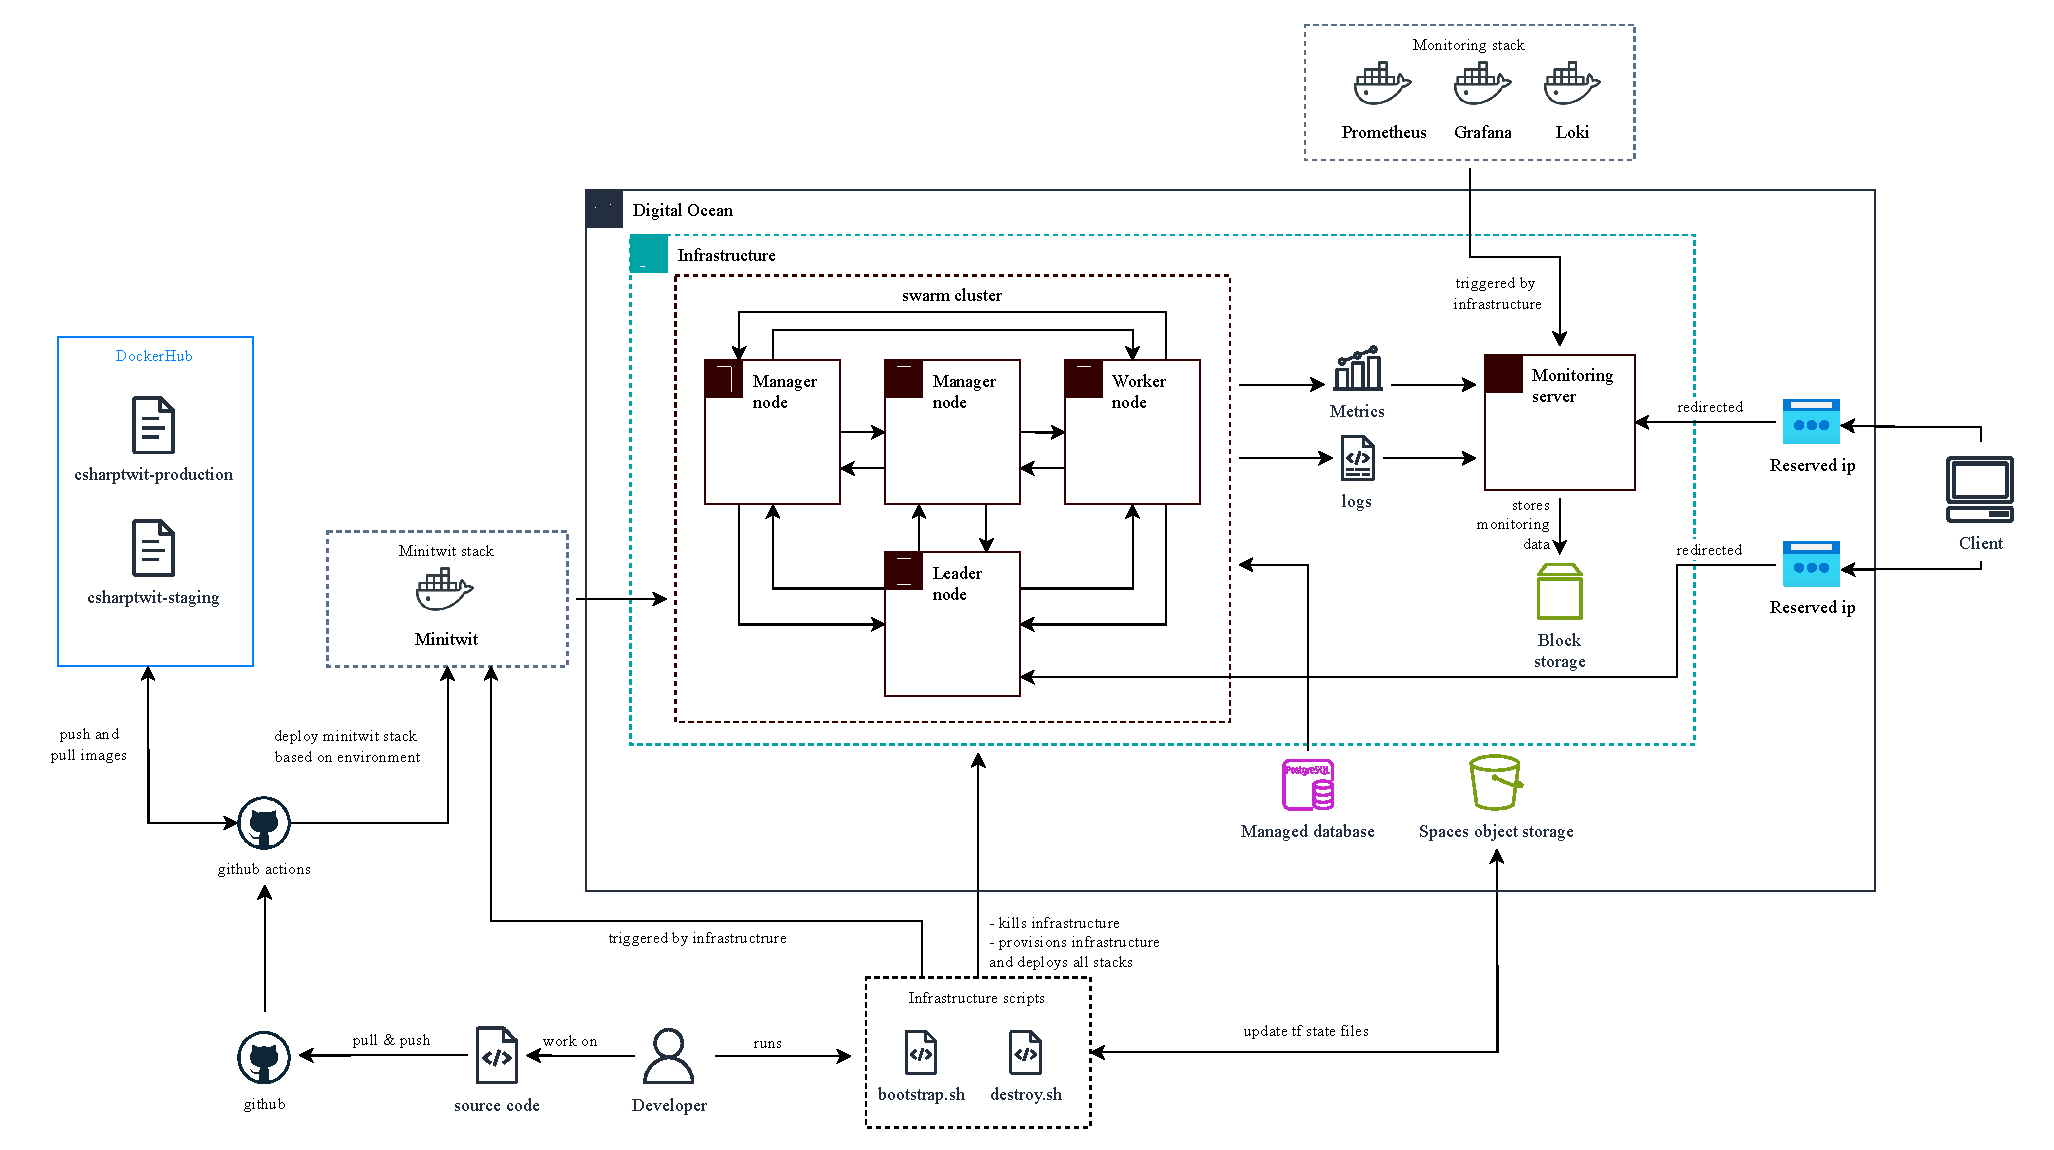
\includegraphics[height=0.8\textwidth, angle=90]{figures/devops-architecture-architecture_v2.pdf}
    \caption{Systems architecture diagram}
    \label{fig:systems-architecture}
\end{figure}


\begin{figure}[t!]
  \begin{center}
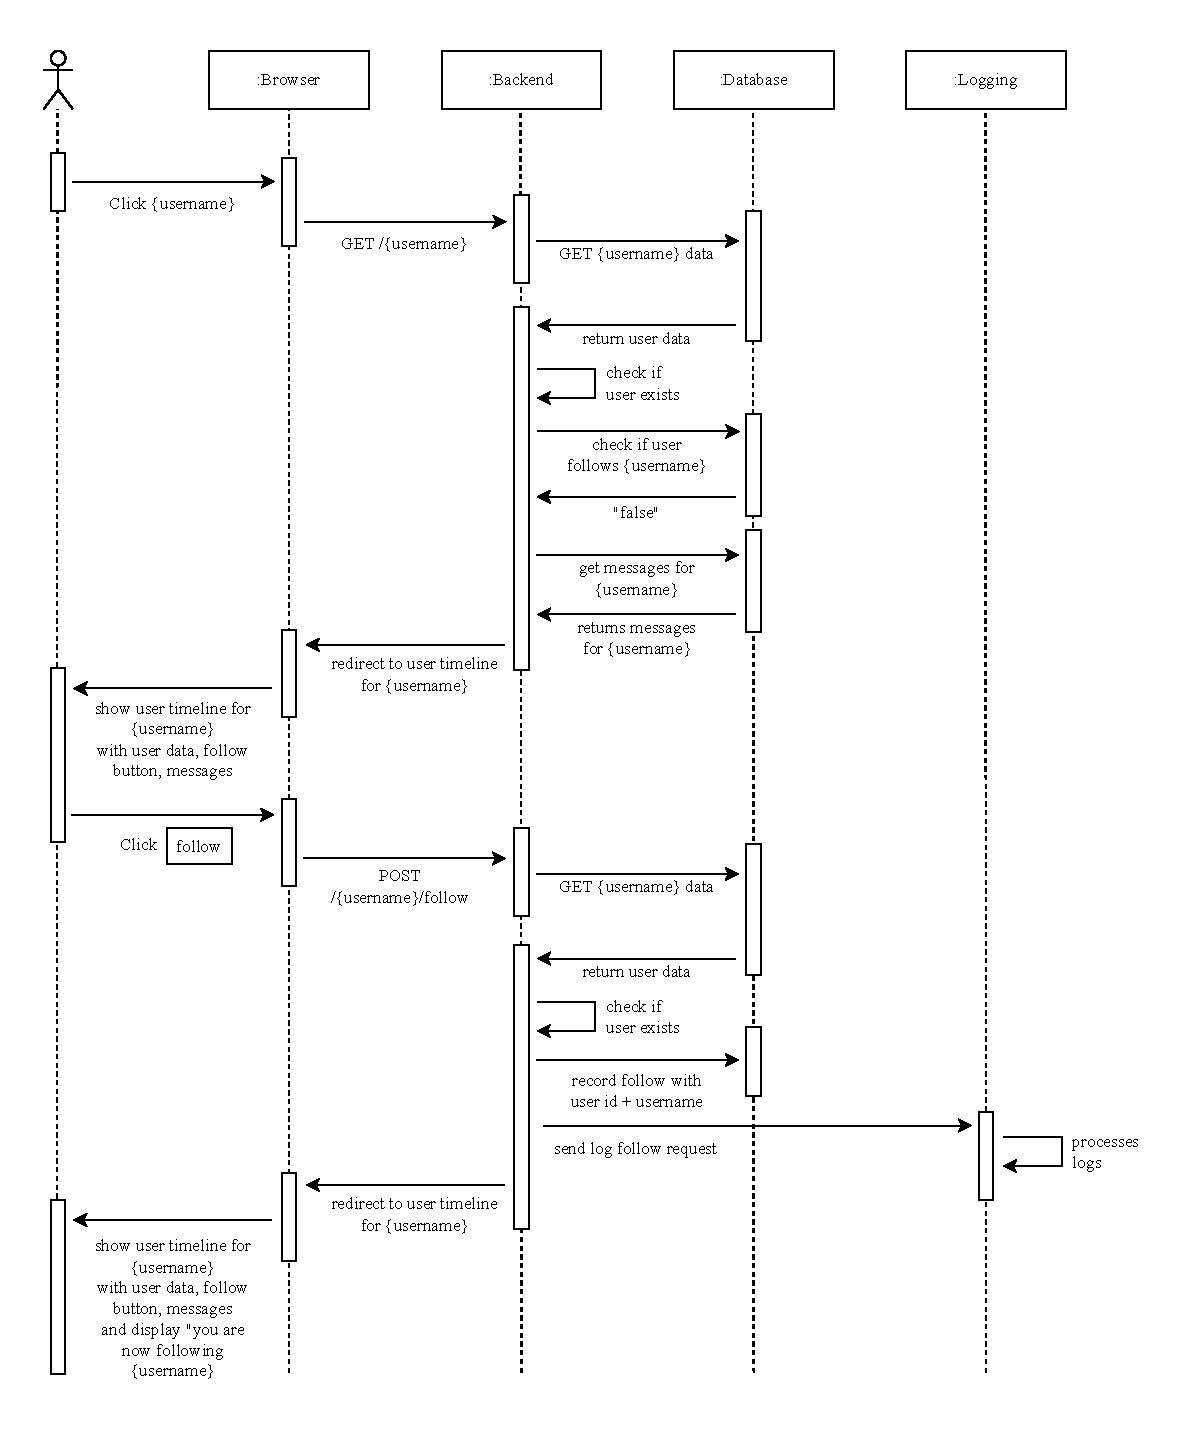
\includegraphics[width=\textwidth]{figures/Sequence_follow_succes.pdf}
    \caption{Sequence diagram of a successful follow scenario.}
    \label{fig:architecture}
  \end{center}
\end{figure}

\end{document}
